% !TEX TS-program = XeLaTeX
% use the following command:
% all document files must be coded in UTF-8
\documentclass[spanish]{textolivre}
% build HTML with: make4ht -e build.lua -c textolivre.cfg -x -u article "fn-in,svg,pic-align"

\journalname{Texto Livre}
\thevolume{15}
%\thenumber{1} % old template
\theyear{2022}
\receiveddate{\DTMdisplaydate{2022}{1}{9}{-1}} % YYYY MM DD
\accepteddate{\DTMdisplaydate{2022}{2}{23}{-1}}
\publisheddate{\DTMdisplaydate{2022}{5}{3}{-1}}
\corrauthor{Fabiola Sáez-Delgado}
\articledoi{10.35699/1983-3652.2022.37810}
%\articleid{NNNN} % if the article ID is not the last 5 numbers of its DOI, provide it using \articleid{} commmand 
% list of available sesscions in the journal: articles, dossier, reports, essays, reviews, interviews, editorial
\articlesessionname{articles}
\runningauthor{Rojas-García et al.} 
%\editorname{Leonardo Araújo} % old template
\sectioneditorname{Hugo Heredia Ponce}
\layouteditorname{Daniervelin Pereira}

\title{Análisis de intervenciones educativas con videojuegos en educación secundaria: una revisión sistemática}
\othertitle{Análise de intervenções educativas com videogames no ensino médio: uma revisão sistemática}
\othertitle{The analysis of educational interventions with video games in secondary education: a systematic review}
% if there is a third language title, add here:
%\othertitle{Artikelvorlage zur Einreichung beim Texto Livre Journal}

\author[1]{Paula Rojas-García \orcid{0000-0001-5549-3162} \thanks{Email: \url{projas@magisteredu.ucsc.cl}}}
\author[2]{Fabiola Sáez-Delgado \orcid{0000-0002-7993-5356} \thanks{Email: \url{fsaez@ucsc.cl}}}
\author[3]{María Graciela Badilla-Quintana \orcid{0000-0002-1317-9228} \thanks{Email: \url{mgbadilla@ucsc.cl}}}
\author[3]{Laura Jiménez-Pérez \orcid{0000-0001-6697-5765} \thanks{Email: \url{ljimenez@ucsc.cl}}}
\affil[1]{Universidad Católica de la Santísima Concepción, Facultad de Educación, Programa de Magíster en Ciencias de la Educación, Concepción, Chile.}
\affil[2]{Universidad Católica de la Santísima Concepción, Facultad de Educación, Centro de Investigación en Educación y Desarrollo CIEDE-UCSC, Departamento Fundamentos de la Pedagogía, Concepción, Chile.}
\affil[3]{Universidad Católica de la Santísima Concepción, Facultad de Educación, Centro de Investigación en Educación y Desarrollo CIEDE-UCSC, Departamento de Currículum , Evaluación y Tecnologías de la Información, Concepción, Chile.}


\addbibresource{article.bib}
% use biber instead of bibtex
% $ biber article

% used to create dummy text for the template file
\definecolor{dark-gray}{gray}{0.35} % color used to display dummy texts
\usepackage{lipsum}
\SetLipsumParListSurrounders{\colorlet{oldcolor}{.}\color{dark-gray}}{\color{oldcolor}}

% used here only to provide the XeLaTeX and BibTeX logos
\usepackage{hologo}

% if you use multirows in a table, include the multirow package
\usepackage{multirow}

% provides sidewaysfigure environment
\usepackage{rotating}

% CUSTOM EPIGRAPH - BEGIN 
%%% https://tex.stackexchange.com/questions/193178/specific-epigraph-style
\usepackage{epigraph}
\renewcommand\textflush{flushright}
\makeatletter
\newlength\epitextskip
\pretocmd{\@epitext}{\em}{}{}
\apptocmd{\@epitext}{\em}{}{}
\patchcmd{\epigraph}{\@epitext{#1}\\}{\@epitext{#1}\\[\epitextskip]}{}{}
\makeatother
\setlength\epigraphrule{0pt}
\setlength\epitextskip{0.5ex}
\setlength\epigraphwidth{.7\textwidth}
% CUSTOM EPIGRAPH - END

% LANGUAGE - BEGIN
% ARABIC
% for languages that use special fonts, you must provide the typeface that will be used
% \setotherlanguage{arabic}
% \newfontfamily\arabicfont[Script=Arabic]{Amiri}
% \newfontfamily\arabicfontsf[Script=Arabic]{Amiri}
% \newfontfamily\arabicfonttt[Script=Arabic]{Amiri}
%
% in the article, to add arabic text use: \textlang{arabic}{ ... }
%
% RUSSIAN
% for russian text we also need to define fonts with support for Cyrillic script
% \usepackage{fontspec}
% \setotherlanguage{russian}
% \newfontfamily\cyrillicfont{Times New Roman}
% \newfontfamily\cyrillicfontsf{Times New Roman}[Script=Cyrillic]
% \newfontfamily\cyrillicfonttt{Times New Roman}[Script=Cyrillic]
%
% in the text use \begin{russian} ... \end{russian}
% LANGUAGE - END

% EMOJIS - BEGIN
% to use emoticons in your manuscript
% https://stackoverflow.com/questions/190145/how-to-insert-emoticons-in-latex/57076064
% using font Symbola, which has full support
% the font may be downloaded at:
% https://dn-works.com/ufas/
% add to preamble:
% \newfontfamily\Symbola{Symbola}
% in the text use:
% {\Symbola }
% EMOJIS - END

% LABEL REFERENCE TO DESCRIPTIVE LIST - BEGIN
% reference itens in a descriptive list using their labels instead of numbers
% insert the code below in the preambule:
%\makeatletter
%\let\orgdescriptionlabel\descriptionlabel
%\renewcommand*{\descriptionlabel}[1]{%
%  \let\orglabel\label
%  \let\label\@gobble
%  \phantomsection
%  \edef\@currentlabel{#1\unskip}%
%  \let\label\orglabel
%  \orgdescriptionlabel{#1}%
%}
%\makeatother
%
% in your document, use as illustraded here:
%\begin{description}
%  \item[first\label{itm1}] this is only an example;
%  % ...  add more items
%\end{description}
% LABEL REFERENCE TO DESCRIPTIVE LIST - END


% add line numbers for submission
%\usepackage{lineno}
%\linenumbers

\begin{document}
\maketitle

\begin{polyabstract}
\begin{abstract}
Este artículo tiene por objetivo sistematizar información empírica sobre las intervenciones de videojuegos educativos en el nivel de Educación Secundaria, mediante la descripción de los participantes, caracterización de la variable independiente, efectividad, limitaciones y proyecciones de los estudios. Para ello, se realizó una revisión sistemática de la literatura, donde se analizaron artículos publicados en las bases de datos Web of Science, Scopus y SciELO, entre los años 2016 y 2021, logrando una muestra final de 19 investigaciones. Los resultados destacan que el continente europeo y concretamente España han desarrollado el mayor número de publicaciones relacionadas con intervenciones de videojuegos en este nivel educativo. Sin embargo, se utilizaron muestras poco representativas. También, se evidenció que se utilizan principalmente estrategias pedagógicas vinculadas al área de las matemáticas para integrar la tecnología al aula, dejando de lado la promoción del área humanista en relación con esta herramienta digital. Finalmente, todas las intervenciones mostraron efectividad; no obstante, se requiere avanzar en esta línea de investigación que está en un nivel de desarrollo incipiente en la educación secundaria, considerando los beneficios que mostraron para propósitos educativos. En conclusión, las intervenciones que incluyen tecnologías en contextos escolares obtienen resultados positivos en el proceso de enseñanza–aprendizaje, ayudando a desarrollar tanto contenidos como habilidades transversales en los educandos.

\keywords{Tecnologías de la información y comunicación \sep Videojuegos educativos \sep Revisión sistemática \sep Educación secundaria \sep Intervenciones}
\end{abstract}

\begin{portuguese}
\begin{abstract}
Este artigo tem como objetivo sistematizar informações empíricas sobre intervenções de videogames educativos no Ensino Médio, por meio da descrição dos participantes, caracterização da variável independente, efetividade, limitações e projeções dos estudos. Para isso, foi realizada uma revisão sistemática da literatura, em que foram analisados artigos publicados nas bases de dados Web of Science, Scopus e SciELO, entre os anos de 2016 e 2021, alcançando uma amostra final de 19 investigações. Os resultados destacam que o continente europeu e especificamente a Espanha têm desenvolvido o maior número de publicações relacionadas a intervenções em videogames nesse nível educacional. No entanto, foram utilizadas amostras não representativas. Além disso, evidenciou-se que as estratégias pedagógicas ligadas à área da matemática são utilizadas principalmente para integrar a tecnologia na sala de aula, deixando de lado a promoção da área humanística em relação a essa ferramenta digital. Por fim, todas as intervenções mostraram eficácia; porém, é preciso avançar nessa linha de pesquisa, que se encontra em um nível incipiente de desenvolvimento no ensino médio, considerando os benefícios que apresentaram para fins educacionais. Em conclusão, as intervenções que incluem tecnologias em contextos escolares obtêm resultados positivos no processo de ensino-aprendizagem, ajudando a desenvolver tanto conteúdos como competências transversais pelos alunos.

\keywords{Tecnologias de informação e comunicação \sep Videogames educativos \sep Revisão sistemática \sep Ensino médio \sep Intervenções}
\end{abstract}
\end{portuguese}

\begin{english}
\begin{abstract}
The aim of this article is to systematize empirical information on educational video game interventions at the Secondary Education level, by describing the participants, characterization of the independent variable, effectiveness, limitations and projections of the studies. For this purpose, a systematic literature review was conducted, in which articles published in the Web of Science, Scopus and SciELO databases were analyzed, between 2016 and 2021, achieving a final sample of 19 studies. The results showed that the European continent, specifically Spain, is the place where most interventions with video games are developed at this educational level. However, the samples used were not very representative. Also, it was shown that pedagogical strategies linked to the area of Mathematics are mainly used to integrate technology into the classroom, leaving aside the promotion of the humanistic area in relation to this digital tool. Finally, all the interventions showed effectiveness; however, it is necessary to advance in this line of research, which is at an incipient level of development in schools, even more so considering the effectiveness they showed for educational purposes. In conclusion, interventions that include technologies in school contexts obtain positive results in the teaching-learning process, helping to develop both content and transversal skills in students.

\keywords{Information and communication technologies \sep Educational video games \sep Systematic review \sep Secondary education \sep Interventions}
\end{abstract}
\end{english}
% if there is another abstract, insert it here using the same scheme
\end{polyabstract}

\section{Introducción}\label{sec-intro}
El sistema educativo se ha visto influenciado por el gran avance de las Tecnologías de la Información y Comunicación (en adelante TIC), las que actúan como un medio que contribuye al desarrollo del proceso de enseñanza–aprendizaje \cite{martinez_soto_evaluacion_2018}. Las TIC son definidas como recursos, herramientas o programas que se utilizan para procesar, administrar y compartir información mediante diversos soportes tecnológicos, siendo caracterizadas por ser interactivas, instantáneas, innovadoras e inmateriales \cite{cervantes_cabello_incursionando_2020,recio_formacion_2016,sanchez-otero_estrategias_2019}. Estas, ofrecen múltiples oportunidades para autorregular o facilitar el aprendizaje, retroalimentar continuamente y promover la reflexión individual \cite{corral_carrillo_recursos_2016}. Actualmente, se tiene a disposición de la educación un amplio espectro de recursos tecnológicos que se pueden implementar, entre ellos, el videojuego educativo, el cual permite combinar el aprendizaje, la información y la colaboración \cite{santa_videojuego_2018}. Esto deja en evidencia que su uso ha traspasado la barrera del entretenimiento y se ha expandido a diversas áreas del conocimiento.

Los videojuegos educativos pueden definirse como un software o entorno virtual de entretenimiento autosuficiente, que tiene implícito un contenido educativo específico e integra los requerimientos tanto lúdicos como formativos, identificando aprendizajes en cada actividad realizada \cite{alvarez_serious_2007,padilla_metodologipara_2011,adell_proceso_2018}. Estos, representan un cambio de paradigma en la forma tradicional que se conciben los juegos, pues se relaciona con algún aspecto de la realidad, que permite al estudiante identificarse a través de una simulación virtual que no implica algún tipo de riesgo para su integridad \cite{urquidi_martin_juegos_2015,lopez_raventos_videojuego_2016}. Como recurso de aula, facilita el desarrollo de habilidades sociales, mejora el rendimiento escolar, desarrolla habilidades cognitivas, motiva el aprendizaje \cite{jimenez_uso_2016}, fomenta la competencia digital y estimula las inteligencias múltiples y la creatividad \cite{grande_de_prado_beneficios_2018}.

Para que un videojuego sea considerado educativo requiere incluir reglas (delimitar lo que el jugador puede o no hacer dentro del juego); metas y objetivos (establecer los retos y los pasos para llegar al punto final); narrativa (contar una historia); y fantasía (poseer escenarios, elementos, personajes o recompensas que estimulen la imaginación, emociones y motivación de los participantes) \cite{pineda_videojuego_2019}. Además, se identifican tres categorías: (1) juegos de estrategia, los que potencian las habilidades creativas y lógicas que permiten alcanzar un objetivo final; (2) juegos de aventura, basados en la superación de obstáculos y decisiones rápidas para superar los inconvenientes del juego; (3) juegos de simulación, los que permiten al jugador desenvolverse en un ambiente basado en la realidad que representa fenómenos sociales y naturales \cite{maraza_quispe_efectos_2018}. 

Variadas son las investigaciones empíricas que exponen experiencias positivas y beneficiosas gracias a la implementación de videojuegos educativos en el aula. Entre ellas se evidencia la mejora de: la comprensión lectora mediante la ejercitación \cite{castro_maximum_2015}, la práctica de actividad física y alimentación saludable \cite{gonzalez_gonzalez_programa_2016,urquidez_romero_physical_2017}, generación de aprendizaje significativo en diversas áreas del conocimiento (MARAZA et al., 2018), rendimiento académico \cite{macias_ruiz_videojuegos_2020}; y habilidades motrices y rítmicas \cite{abarca_rendimiento_2020}. 

Se han identificado algunas revisiones sistemáticas que abarcan niveles de primaria y Educación Superior, que indagaron sobre su efectividad o se focalizaron en una asignatura específica \cite{araujo_exergames_2017, torres-toukoumidis_desarrollo_2016,diaz_history_2018,sousa_videogames_2018}, pero no se logra identificar revisiones sistemáticas de la literatura sobre la implementación de videojuegos en el nivel de Educación Secundaria, a pesar de la indudable importancia y beneficio en el sistema escolar. Por lo anteriormente expuesto, se planteó la siguiente interrogante ¿Qué características tiene la evidencia empírica sobre la intervención de videojuegos educativos en el nivel de educación secundaria? De la cual derivaron los siguientes objetivos específicos son: 

\begin{enumerate}
    \item Describir a los participantes de estudios que han utilizado videojuegos educativos en el nivel de secundaria, mediante los siguientes aspectos: (a) país de los participantes, (b) y número de participantes. 
    \item Caracterizar la variable independiente de los estudios empíricos que han utilizado videojuegos educativos en el nivel de secundaria, mediante los siguientes aspectos: (a) estrategias pedagógicas seleccionadas, (b) tipos de videojuegos, (c) asignatura donde se realiza la intervención, (d) lugar de implementación, (e) cantidad de sesiones de la intervención.  
    \item Determinar la efectividad de las intervenciones que han utilizado videojuegos educativos en el nivel de secundaria.
    \item Establecer las limitaciones y futuras líneas de investigación de estudios que han utilizado videojuegos educativos en el nivel de secundaria. 
\end{enumerate}

\section{Método}\label{sec-normas}
Se utilizó el método de revisión sistemática exhaustiva de la literatura \cite{estarli_items_2016,sanchez_meca_revisiones_2010}, basado en los lineamientos de PRISMA \cite{page_declaracion_2021} y la dirección de trabajos previos que han utilizado este diseño en educación \cite{saez_revision_2018,lopez-angulo_revision_2020}. 

Además, se incluyeron los dos procesos que conlleva una revisión sistemática. El primero, permite la identificación de la muestra de estudios que se analizarán y está representado por 5 fases (ver \Cref{fig01}). El segundo, implica el método para el análisis de la información de los estudios que fueron incluidos en la revisión. 

\begin{figure}[htbp]
 \centering
 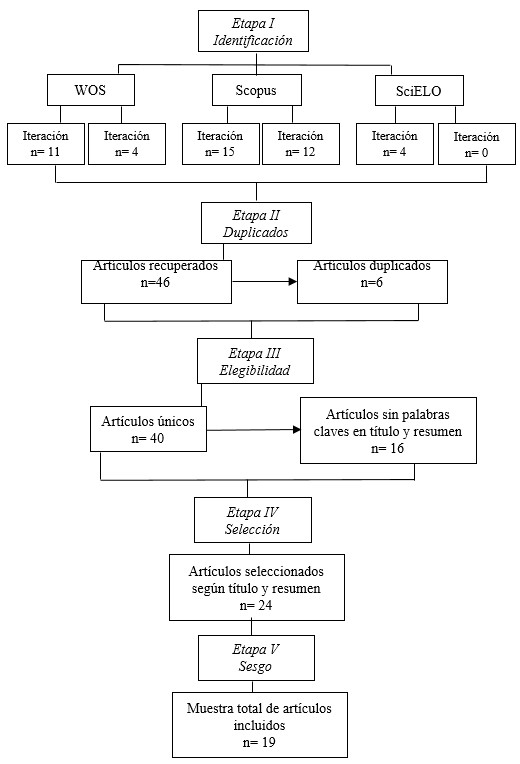
\includegraphics[width=0.85\textwidth]{Fig1.jpg}
 \caption{Diagrama de flujo de la información de las fases de una revisión sistemática.}
 \label{fig01}
 \source{Elaboración propia.}
\end{figure}

\subsection{Proceso 1 del método: identificación de los estudios}\label{sec-conduta}
Fase 1 de identificación. 
Se realizó una exploración electrónica y sistemática de artículos el día 18 de mayo de 2021, mediante la consulta de las bases de datos Web of Science, Scopus y SciELO, empleando los siguientes descriptores en inglés: video game OR serious game OR virtual simulation AND secondary school OR secondary education OR high school OR high school education. Además, para validar el algoritmo de búsqueda, este fue presentado a 3 expertos, doctores del área de la educación y con experiencia en investigación de tecnologías educativas. 

Fase 2 de duplicados. Los registros identificados en las bases de datos se revisaron para descartar aquellos que se encontraban repetidos. 

Fase 3 de cribado. Consistió en la lectura del título y resumen de los estados eliminando aquellos que estaban fuera del foco de esta revisión. 

Fase 4 de selección. Se aplicaron criterios de exclusión, eliminado aquellos estudios que pertenecían a las siguientes categorías: (1) Artículos teóricos, revisiones sistemáticas, meta – análisis; (2) La muestra no son escolares de educación secundaria, es decir son preescolares, estudiantes de primaria, estudiantes con necesidades educativas especiales, adultos, universitarios, profesores, apoderados, directivos; (3) El contexto es distinto al escolar, es decir es clínico, laboral, u otro; (4) No incluye intervenciones con videojuegos educativos en el aula. 

Fase 5: Sesgo. Permitió asegurar la calidad y rigurosidad del estudio, minimizando el sesgo del proceso de selección, a través de la revisión del procedimiento completo por parte de un revisor externo. 

\subsection{Proceso 2 del método: extracción de información}\label{sec-fmt-manuscrito}
Este proceso consistió en definir un protocolo para la extracción de la información de los estudios que fueron seleccionados e incluidos dentro de la investigación (Ver \Cref{tbl1}).

\begin{table}[htpb]
\caption{Aspectos incluidos en matriz de análisis de información para artículos seleccionados.}
\label{tbl1}
\begin{tabular}{llp{7.5cm}}
\toprule 
 & \textbf{Aspecto} & \textbf{Coluna 2}                                      \\ 
\midrule
1.    & ID  & Número de identificación de los artículos organizado por orden alfabético
\\ 
2. & Cita & Apellido de autor/es y año de publicación
\\
3. & País & Indica el país donde se desarrolló el estudio
\\
4. & Título & Indica el título de la investigación
\\
5. & Estrategias & Se identifican las estrategias utilizadas en las intervenciones educativas para aplicarlas al aula
\\
6. & Efectividad & 6.1 Explicita en qué aspecto educativo fue efectiva la intervención

6.2 Indica si logra cumplir con el objetivo propuesto
\\
7. & Videojuego educativo & Indica qué videojuego educativo fue utilizado para la intervención
\\
8. & Descripción del videojuego educativo & Se describe en qué consiste el videojuego y cuál es su función.
\\
9. & Área de implementación & Asignatura o área de implementación de la intervención educativa
\\
10. & Muestra & Cantidad de participantes incluidos en la muestra
\\
11.  & Futuras líneas de investigación & Indica las futuras líneas de investigación declaradas en el estudio
\\
12. & Limitaciones & Indica las limitaciones declaradas en el estudio
\\
13. & Sesiones & Indica la cantidad de sesiones que se implementaron el aula con el videojuego educativo.
\\
\bottomrule
\end{tabular}
\source{Elaboración propia.}
\end{table}

El detalle de la matriz de extracción y las diversas fases del proceso de la presente revisión sistemática, se pueden observar en el siguiente link de repositorio externo (\url{https://figshare.com/s/80f28374f8bc5c6c7c0c}).


\section{Resultados}\label{sec-formato}

\subsection{Resultado del Objetivo 1. Descripción de los participantes}

\subsubsection{Resultados respecto del país de los participantes del estudio}

Respecto al país de los participantes, los resultados mostraron que España es el más frecuente (32 \%), seguido por Estados Unidos (22 \%) y por Países Bajos (11 \%). A partir de esto, se establecieron 4 categorías en correspondencia con la región del mundo, en la cual la región europea (63 \%) mostró más estudios, seguida de América del Norte (27 \%). Además, se identificó solo un estudio en América Latina (Ver \Cref{tbl2}). 

\begin{table}[htbp]
\caption{País de los participantes de los estudios.}
\label{tbl2}
\centering
\begin{tabular}{l l l l l l l}
\toprule 
\textbf{País} & \textbf{ID} & \textbf{N} & \textbf{\%} & \textbf{Región del mundo} & \textbf{N} & \textbf{\%}
\\
\midrule
E.E.U.U & 1,9,10,11 & 4 & 22 \% & \multirow{2}{*}{América del norte} & \multirow{2}{*}{5} & \multirow{2}{*}{27 \%}
\\
México & 16 & 1 & 5 \% & & &
\\
España & 2,4,7,12,13,15 & 6 & 32 \% & \multirow{6}{*}{Europa} & \multirow{6}{*}{12} & \multirow{6}{*}{63 \%}
\\
Portugal & 3 & 1 & 5 \% & & &
\\
Países bajos & 5,19 & 2 & 11 \% & & &
\\
Multicultural & 8 & 1 & 5 \% & & &
\\
Italia & 6 & 1 & 5 \% & & &
\\
Grecia & 17 & 1 & 5 \% & & &
\\
Colombia & 14 & 1 & 5 \% & Latinoamérica & 1 & 5 \%
\\
China & 18 & 1 & 5 \% & Asia & 1 & 5 \%
\\
\bottomrule
\end{tabular}
\source{Elaboración propia.}
\end{table}

\subsubsection{Resultados del tamaño de la muestra considerada en los estudios}\label{sec-modelo}
De acuerdo con los tamaños muestrales identificados en los estudios, estos se agruparon en rangos de cada 100. Considerando el máximo del tamaño de la muestra, se constituyeron seis rangos de cantidad, siendo los más frecuentes los que incluían intervenciones entre 1 a 100 estudiantes participantes (53 \%) y 101 a 200 estudiantes participantes (21 \%) (Ver \Cref{tbl3}).
 
\begin{table}[htbp]
\caption{Tamaño de la muestra en la intervención con videojuegos educativos.}
\label{tbl3}
\centering
\begin{tabular}{l l l l}
\toprule 
\textbf{Tamaño de la muestra} & \textbf{ID} & \textbf{N} & \textbf{\%}
\\
\midrule
1 - 100 estudiantes & 1,4,9,10,12,13,15,16,17,18 & 10 & 53 \%
\\
101 - 200 estudiantes & 5,6,7,19 & 4 & 21 \%
\\
201 - 300 estudiantes & 14 & 1 & 5 \%
\\
301 - 400 estudiantes & 2,11 & 2 & 11 \%
\\
401 - 500 estudiantes & 3 & 1 & 5 \%
\\
501 o más estudiantes & 8 & 1 & 5 \%
\\
\bottomrule
\end{tabular}
\source{Elaboración propia.}
\end{table}


\subsection{Resultado del Objetivo 2. Características de la variable independiente}\label{sec-organizacao}

\subsubsection{Resultados de las estrategias pedagógicas utilizadas con los videojuegos educativos}
De acuerdo a las estrategias pedagógicas seleccionadas para que la aplicación del videojuego generara un conocimiento, habilidad o destreza efectiva en los educandos, se identificaron un total de 17 estrategias utilizadas dentro del presente estudio. Estas, se categorizaron en seis grupos según su finalidad: Aprendizaje basado en métodos matemáticos, métodos de evaluación user experience, sesiones de entrenamiento, estrategias para la comprensión y el aprendizaje de la ciencia, aprendizaje visual y aprendizaje y creación mediante el juego; siendo la más frecuente el aprendizaje basado en métodos matemáticos (37 \%) (Ver \Cref{tbl4}).

\begin{table}[htbp]
\caption{Estrategias pedagógicas utilizadas para la incorporación de videojuegos educativos.}
\label{tbl4}
\centering
\begin{tabular}{p{4.5cm} l l l p{3.9cm} l l}
\toprule 
\textbf{Estrategia} & \textbf{ID} & \textbf{N} & \textbf{\%} & \textbf{Agrupación de estrategias} & \textbf{N} & \textbf{\%}
\\
\midrule
Aprendizaje basado en casos (CBL) & 1 & 1 & 5 \% & \multirow{6}{=}{Aprendizaje basado en métodos matemáticos} & \multirow{6}{*}{7} & \multirow{6}{*}{37 \%}
\\
Aprendizaje basado en problemas matemáticos & 2 & 1 & 5 \% & & &
\\
Resolución de métodos matemáticos a través del método Polya & 4 & 1 & 5 \% & & & 
\\
Aprendizaje basado en problemas (ABP) con temáticas STEM & 8,9 & 2 & 11 \% & & & 
\\
Razonamiento basado en casos (CBR) & 14 & 1 & 5 \% & & & 
\\
Aprendizaje basado en el razonamiento lógico-matemático & 16 & 1 & 5 \% & & & 
\\
Método de evaluación User Experience (UX) & 3 & 1 & 5 \% & Método de evaluación user experience (UX) & 1 & 5 \%
\\
Sesiones de entrenamiento cognitivo basadas en el paradigma de la señal parada (SST) & 5 & 1 & 5 \% & \multirow{4}{*}{Sesiones de entrenamiento} & \multirow{4}{*}{4} & \multirow{4}{*}{21 \%}
\\
Programa de entrenamiento de inteligencia emocional (IE) basado en el modelo de habilidades de Mayer and Salovey & 6 & 1 & 5 \% & & & 
\\
Entrenamiento modelado del comportamiento & 10 & 1 & 5 \% & & & 
\\
Marco de integración del comportamiento & 11 & 1 & 5 \% & & &
\\
Metas epistémicas para desarrollar la comprensión de conceptos y variables científicas & 7 & 1 & 5 \% & \multirow{2}{=}{Estrategias para la comprensión y el aprendizaje de la ciencia} & \multirow{2}{*}{2} & \multirow{2}{*}{11 \%}
\\
Enfoque constructivista del aprendizaje de la ciencia & 18 & 1 & 5 \% & & &
\\
Aprendizaje visual & 13 & 1 & 5 \% & Aprendizaje visual & 1 & 5 \%
\\
Creación de videojuego & 12 & 1 & 5 \% & \multirow{3}{=}{Aprendizaje y creación mediante el juego} & \multirow{3}{*}{4} & \multirow{3}{*}{21 \%}
\\
Aprendizaje activo mediante la gamificación & 15 & 1 & 5 \% & & &
\\
Aprendizaje basado en juegos (Game based learning, GBL) & 17,19 & 2 & 11 \% & & &
\\
Total: & & 19 & 100 \% & Total: & 19 & 100 \%
\\
\bottomrule
\end{tabular}
\source{Elaboración propia.}
\end{table}

\subsubsection{Resultados según el tipo de videojuego educativo}\label{sec-organizacao-latex}
En cuanto al tipo de videojuego utilizado dentro de la intervención educativa, se detectó que los 19 estudios trabajaron con videojuegos diferentes. A raíz de esto, los resultados se agruparon en tres categorías: acceso del videojuego, categoría del videojuego y tipo de videojuego.

La primera categoría evidencia que mayoritariamente, los videojuegos utilizados son de libre acceso (58 \%) (Ver \Cref{tbl5}).

\begin{table}[htbp]
\caption{Acceso de los videojuegos educativos.}
\label{tbl5}
\centering
\begin{tabular}{l l l l}
\toprule 
\textbf{Acceso al videojuego} & \textbf{ID} & \textbf{N} & \textbf{\%}
\\
\midrule
Libre Acceso & 1,2,4,6,7,8,12,13,16,17,18 & 11 & 58 \%
\\
Pagado & 5,11 & 2 & 11 \%
\\
No se declara & 3,10,14,15,19,9 & 6 & 32 \%
\\
Total & & 19 & 100 \%
\\
\bottomrule
\end{tabular}
\source{Elaboración propia.}
\end{table}

Según la segunda categoría, los videojuegos implementados tienen frecuentemente un fin educativo (58 \%) (Ver \Cref{tbl6}).

\begin{table}[htbp]
\caption{Categoría de los videojuegos educativos.}
\label{tbl6}
\centering
\begin{tabular}{l l l l}
\toprule 
\textbf{Categoría del videojuego} & \textbf{ID} & \textbf{N} & \textbf{\%}
\\
\midrule
Comercial & 2,4,6,7,11,12,13 & 7 & 37 \%
\\
Educativo & 1,3,8,9,10,14, 15,16,17,18,19 & 11 & 58 \%
\\
No se declara & 5 & 1 & 5 \%
\\
Total & & 19 & 100 \%
\\
\bottomrule
\end{tabular}
\source{Elaboración propia.}
\end{table}

Respecto a los tipos de videojuegos más utilizados en las intervenciones, estos son los de simulación (37 \%) y los multiplataforma (26 \%) (Ver \Cref{tbl7}).

\begin{table}[htbp]
\caption{Tipo de videojuegos educativos.}
\label{tbl7}
\centering
\begin{tabular}{l l l l}
\toprule 
\textbf{Tipo de videojuego} & \textbf{ID} & \textbf{N} & \textbf{\%}
\\
\midrule
Juego de rol & 13,16 & 2 & 11 \%
\\
Juego de simulación & 1,3,5,8,10,11,18 & 7 & 37 \%
\\
Juego de estrategia & 2,7 & 2 & 11 \%
\\
Juego inmersivo & 9 & 1 & 5 \% 
\\
Multiplataforma & 4,6,12,14,17 & 5 & 26 \%
\\
Trivia & 15 & 1 & 5 \%
\\
Aplicación móvil & 16 & 1 & 5 \%
\\
Total & & 19 & 100 \%
\\
\bottomrule
\end{tabular}
\source{Elaboración propia.}
\end{table}

%Há um erro de soma na coluna N. Pedi para a autora verificar.

\subsubsection{Resultados según la asignatura de implementación del videojuego educativo}\label{sec-titulo}
Respecto a las asignaturas de implementación del videojuego educativo, se concluye que las más frecuentes son matemáticas (32 \%) y formación general (21 \%). A raíz de esto, se establecieron tres categorías según el área disciplinar de desarrollo propuesta por \textcite{de_frascati_manual_2015}, en donde el área de las ciencias naturales (58 \%), es la más utilizada en la aplicación, en contraste con el área humanista (16 \%) que se presenta como la menos habitual (Ver \Cref{tbl8}).

\begin{table}[htbp]
\caption{Asignatura de aplicación de los videojuegos educativos.}
\label{tbl8}
\centering
\begin{tabular}{ p{3.5cm} l l l l l l}
\toprule 
\textbf{Asignatura de aplicación videojuego} & \textbf{ID} & \textbf{N} & \textbf{\%} & \textbf{Áreas disciplinares} & \textbf{N} & \textbf{\%}
\\
\midrule
Biología & 1,18 & 2 & 11 \% & \multirow{5}{*}{Ciencias naturales} & \multirow{5}{*}{11} & \multirow{5}{*}{58 \%}
\\
Física & 7 & 1 & 5 \% & & &
\\
Química & 11 & 1 & 5 \% & & &
\\
Matemáticas & 2,4,9,14,16,19 & 6 & 32 \% & & &
\\
Computación y ciencias de la información & 17 & 1 & 5 \% & & &
\\
Historia & 3 & 1 & 5 \% & \multirow{3}{*}{Humanidades} & \multirow{3}{*}{3} & \multirow{3}{*}{16 \%}
\\
Artes visuales & 12 & 1 & 5 \% & & &
\\
Filosofía & 13 & 1 & 5 \% & & &
\\
Economía & 15 & 1 & 5 \% & Ciencias sociales & 5 & 26 \%
\\
Total & & 19 & 100 \% & Total & 19 & 100 \%
\\
\bottomrule
\end{tabular}
\source{Elaboración propia.}
\end{table}

\subsubsection{Resultados de las sesiones de intervención}\label{sec-idioma}
De acuerdo con el número de sesiones de intervención realizadas, se agruparon por rangos de 5. De acuerdo con esto el rango de 1 a 5 sesiones fue el más frecuente (32 \%), mientras que el rango de 20 o más sesiones fue el menos recurrente (5 \%) en los estudios (Ver \Cref{tbl9}).

\begin{table}[htbp]
\caption{Cantidad de sesiones de intervención con los videojuegos educativos.}
\label{tbl9}
\centering
\begin{tabular}{p{4cm} l l l}
\toprule 
\textbf{Cantidad de sesiones} & \textbf{ID} & \textbf{N} & \textbf{\%}
\\
\midrule
1 a 5 sesiones & 5,8,9,10,18,19 & 6 & 32 \%
\\
6 a 10 sesiones & 3,6,11,12,17 & 5 & 26 \%
\\
11 a 15 sesiones & 0 & 0 & 0 \%
\\
16 a 20 sesiones & 2,4,7 & 3 & 16 \%
\\
20 o más sesiones & 14 & 1 & 5 \%
\\
No se declara la cantidad de sesiones & 1,13,15,16 & 4 & 21 \%
\\
Total & & 19 & 100 \%
\\
\bottomrule
\end{tabular}
\source{Elaboración propia.}
\end{table}

\subsubsection{Resultados según lugar de aplicación de la intervención}
Según el lugar de aplicación de la intervención, los resultados muestran que dentro del aula regular fue donde mayoritariamente se implementaron los videojuegos educativos (58 \%) (ver \Cref{fig02}).

\begin{figure}[htbp]
 \centering
 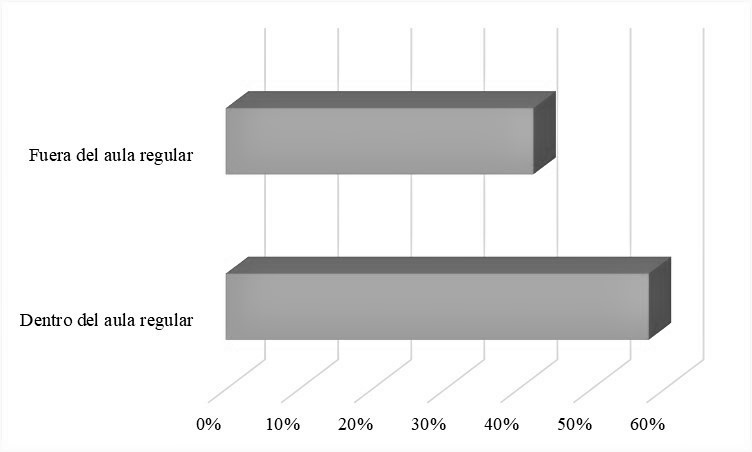
\includegraphics[width=0.85\textwidth]{Fig2.jpg}
 \caption{Lugar de aplicación de la intervención.}
 \label{fig02}
 \source{Elaboración propia.}
\end{figure}

\subsection{Resultados del objetivo 3.  Efectividad de las intervenciones con videojuegos educativos}\label{sec-secoes}
En relación a la efectividad de los videojuegos educativos, los resultados evidencian que mayoritariamente suelen ser efectivos en su totalidad (84 \%) (ver \Cref{fig03}). Además, las variables más trabajadas son las que se relacionan con el aumento del aprendizaje en una asignatura o área específica (53 \%) y la mejora motivación y desarrollo de habilidades del educando (32 \%) (Ver \Cref{tbl10}).

\begin{table}[htbp]
\caption{Variables de la efectividad de los videojuegos educativos.}
\label{tbl10}
\centering
\begin{tabular}{p{7.7cm} l l l}
\toprule 
\textbf{Variable de la efectividad} & \textbf{ID} & \textbf{N} & \textbf{\%}
\\
\midrule
Aumento de aprendizaje en asignatura/ área específica & 1,2,9,11,12,14,16,17,18, 19 & 10 & 53 \%
\\
Mejora motivación y desarrollo de habilidades & 3,5,6,8,13,15 & 6 & 32 \%
\\
Mejora de competencias & 4,7 & 2 & 11 \%
\\
Mejora de la autoeficacia y percepción del conocimiento & 10 & 1 & 5 \%
\\
Total & & 19 & 100 \%
\\
\bottomrule
\end{tabular}
\source{Elaboración propia.}
\end{table}

\begin{figure}[htbp]
 \centering
 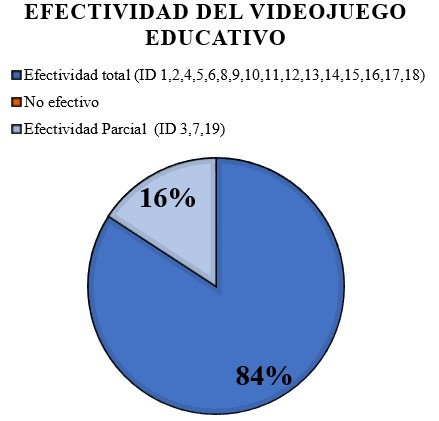
\includegraphics[width=0.65\textwidth]{Fig3.jpg}
 \caption{Efectividad de los videojuegos educativos en educación secundaria.}
 \label{fig03}
 \source{Elaboración propia.}
\end{figure}


\subsection{Resultados del objetivo 4. Limitaciones y proyecciones declaradas en los estudios}\label{sec-format-simple}

\subsubsection{Resultados de las limitaciones declaradas en los estudios}\label{sec-format-simple}

En los 19 estudios analizados, se identificó que 5 de ellos no declararon sus limitaciones. De los 14 restantes que, si las declararon, se evidenció un total de 21 limitaciones, pues algunos expusieron más de una en sus artículos, de las cuales derivaron tres categorías: Limitaciones de la muestra, se relacionan con las características y tamaños muestrales; limitaciones de la intervención, son aquellas que declaran problemáticas con el diseño, alcance o método investigativo; y limitaciones económicas, se relacionan netamente con lo monetario. 

A raíz de esto, se concluye que las mayores limitaciones que presentaron los trabajos son en relación con la propia intervención realizada (42 \%), es decir, en su aplicación, diseño u otro elemento. Mientras que las limitaciones menos frecuentes, son las económicas (8 \%) (Ver \Cref{tbl11}).

\begin{table}[htbp]
\caption{Limitaciones declaradas en los estudios analizados.}
\label{tbl11}
\centering
\begin{tabular}{l l l l}
\toprule 
\textbf{Limitaciones de los estudios} & \textbf{ID} & \textbf{N} & \textbf{\%}
\\
\midrule
Limitaciones de la muestra & 1,4,5,6,9,10,16,17 & 8 & 31 \%
\\
Limitaciones de la intervención & 1,3,5,7,8,9,10,11,17,18,19 & 11 & 42 \%
\\
Limitaciones económicas & 3,11 & 2 & 8 \%
\\
No se declaran limitaciones & 2,12,13,14,15 & 5 & 19 \%
\\
Total & & 26 & 100 \%
\\
\bottomrule
\end{tabular}
\source{Elaboración propia.}
\end{table}

\subsubsection{Resultados de las futuras líneas de investigación declaradas en los estudios}\label{sec-format-simple}

Del total de estudios analizados, se identificó que 4 de ellos no declararon la proyección de sus trabajos en futuras líneas de investigación. Los demás estudios que si las declararon (n=15), evidenciaron un total de 28 proyecciones, pues algunos expusieron más de una en sus artículos. Estas se agruparon en cuatro categorías, según los elementos manifestados para incorporar en sus futuros trabajos: muestra, diseño, intervención e instrumento. A raíz de esto, se concluye que las futuras líneas de investigación más declaradas se asocian a la misma intervención (38 \%) y al método del estudio (31 \%). Mientras que la menos frecuente es el tipo de instrumento utilizado en la investigación (3 \%) (Ver \Cref{tbl12}).

\begin{table}[htbp]
\caption{Futuras líneas de investigación declaradas en los estudios analizados.}
\label{tbl12}
\centering
\begin{tabular}{l l l l}
\toprule 
\textbf{Futuros trabajos} & \textbf{ID} & \textbf{N} & \textbf{\%}
\\
\midrule
Muestra & 1,10,11,16,18 & 5 &16 \%
\\
Diseño & 1,3,5,6,9,9,11,11,17,17 & 10 & 31 \%
\\
Intervención & 2,3,6,7,12,14,16,17,17,17,18,19 & 12 & 38 \%
\\
Instrumento & 12 & 1 & 3 \%
\\
No declara & 4,8,13,15 & 4 & 13 \%
\\
Total & & 32 & 100 \%
\\
\bottomrule
\end{tabular}
\source{Elaboración propia.}
\end{table}

\section{Discusión}\label{sec-links}

\subsection{Discusión del objetivo 1. Descripción de los participantes}

\subsubsection{Discusión del país de los participantes del estudio}
La presente investigación encontró en sus resultados, que el país donde más se desarrollan intervenciones educativas con videojuegos fue en España (32 \%), lo que evidencia que el continente europeo se posiciona como el más productivo (65 \%) en esta línea de investigación. Esto es coherente con revisiones previas \cite{gonzalez-sancho_estado_2019,baranowski_descriptive_2020} y con lo que señalan \textcite{aznar_diaz_tecnologimovil_2018,maraza_quispe_efectos_2018,collado_sector_2018}, sobre el aumento, auge y consumismo tecnológico que se desarrolla en esta región del mundo. Esto conlleva no solo a un uso de tecnologías con objetivos de entretenimiento, sino que su incremento, también estaría progresando el plano educativo, con propósitos pedagógicos y de aprendizaje \cite{nunez-barriopedro_videojuegos_2020}. 

En contraste a este resultado, se refleja la carente productividad de intervenciones en los países Latinoamericanos, pues solo un estudio se realizó en Colombia (5 \%) y no se identificó ninguno implementado en Chile. Esto evidencia la escasa inclusión, estimulación e investigación de las TIC dentro los procesos de enseñanza aprendizaje en los niveles de secundaria del continente, y sobre todo, en el sistema escolar chileno. A raíz de lo anteriormente mencionado, es que Latinoamérica podría incorporar intervenciones con videojuegos en sus programas de mejora educativa, pues según toda la evidencia empírica expuesta en la presente investigación, se pueden lograr mejoras significativas, siempre y cuando los recursos sean implementados con estrategias pertinentes a los objetivos propuestos y contextualizados a la realidad de cada establecimiento. 

\subsection{Discusión respecto de los resultados del tamaño de la muestra}\label{sec-outras-estr}
De acuerdo con los resultados de los tamaños muestrales identificados en el estudio, estos se agruparon en rangos de cada 100. Considerando el máximo del tamaño de la muestra, se constituyeron seis rangos de cantidad, en donde los más frecuentes son los que incluían intervenciones entre 1 a 100 estudiantes participantes (53 \%) y 101 a 200 estudiantes participantes (21 \%). En relación con la gran cantidad de estudiantes que alberga un establecimiento educacional, los resultados de este estudio ponen en evidencia la poca representatividad de la muestra, lo que genera un alejamiento respecto a la realidad y excluye a sujetos que podrían aportar una valiosa información. Además, esto se contradice con el tipo de enfoque utilizado en las investigaciones, ya que todos los estudios declararon ser cuantitativos o mixtos, por lo que es esperable que las investigaciones tengan un número robusto de participantes \cite{delice_sampling_2010}. Sin embargo, el tamaño muestral podría denotar una problemática relacionada con la infraestructura tecnológica presente en los establecimientos educacionales, ya que probablemente no se cuente con aparatos tecnológicos para todo el estudiantado, lo que provoca un retraso en el trabajo investigativo y una selección o reducción de la muestra producto de la brecha digital. Esto se refuerza con la idea de \textcite{gomez_navarro_brecha_2018}, pues expone que los procesos innovadores y tecnológicos, se han centrado solo en algunas regiones o países, dejando en evidencia la desigualdad digital que afecta principalmente al sector más pobre de la población.

\subsection{Discusión del objetivo 2. Características de la variable independiente}\label{sec-listas}

\subsubsection{Discusión respecto de los resultados de las estrategias pedagógicas utilizadas con los videojuegos educativos}
Los resultados respecto a las estrategias pedagógicas utilizadas para la aplicación de los videojuegos educativos, denotó que el aprendizaje basado en métodos matemáticos es el más utilizado (37 \%) dentro de las intervenciones, lo que se relaciona directamente con la asignatura de matemáticas, ya que también fue una de las más recurrentes en el presente estudio. Estos resultados denotan que las estrategias pedagógicas utilizadas con mayor frecuencia para implementar el videojuego educativo en el aula, presentan una preferente inclinación hacia la mejora cognitiva de los estudiantes, por sobre el desarrollo de elementos socio-motivacionales que puedan influir dentro del proceso de enseñanza - aprendizaje. Por un lado, lo anteriormente expuesto se refuerza con la revisión sistemática previa de LEÓN et al. (2020), la cual manifiesta que los videojuegos en la asignatura de historia, centran sus estrategias en el desarrollo cognitivo. Por otro lado, existen variados estudios que se contraponen a este hallazgo, pues despliegan estrategias en ambos ámbitos, de forma que se abarque de forma más completa al discente, tanto en el plano del contenido como en lo socioemocional y motivacional \cite{araujo_exergames_2017,torres-toukoumidis_desarrollo_2016,mendez_uso_2021,prieto_andreu_revision_2021}.  A raíz de esto, es que se podría evaluar incorporar en las planificaciones de implementación del videojuego educativo, una estrategia que complemente ambos ámbitos, de forma que el recurso tecnológico sea una experiencia íntegra de aprendizaje y bienestar en el estudiantado. 
Os artigos poderão conter listas numeradas ou não numeradas.

\subsubsection{Discusión respecto de los resultados del tipo de videojuego educativo}\label{sec-figuras-tabelas}
Los resultados respecto a los videojuegos educativos utilizados dentro de los estudios, evidencian que los más utilizados son los de acceso libre (58 \%), que tienen un fin educativo (no comercial) (58 \%) y emplean preferentemente un tipo de videojuego de simulación (37 \%) y multiplataforma (26 \%) (Para graficar mejor lo anteriormente expuesto, (ver \Cref{fig04}). Las dos primeras categorías visibilizan la realidad mundial educativa, pues no todos los establecimientos secundarios tienen los recursos monetarios para comprar videojuegos e implementarlos en el aula. Además, si estos tienen un libre acceso en la web y su finalidad es el ámbito educativo, solo bastaría una previa planificación para lograr la finalidad pedagógica de forma óptima. Esto, se relaciona directamente con estudios a nivel latinoamericano y europeo, pues la población estudiantil se encuentra mayoritariamente en escuelas públicas \cite{murillo_segregacion_2017}. 

\begin{figure}[htbp]
 \centering
 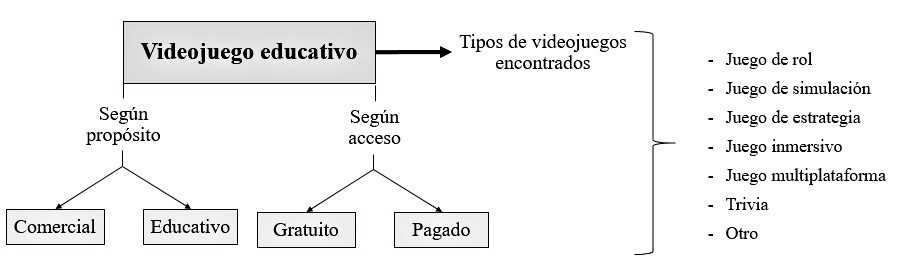
\includegraphics[width=0.95\textwidth]{Fig4.jpg}
 \caption{Tipo de videojuego basado en los hallazgos de este estudio.}
 \label{fig04}
 \source{Elaboración propia.}
\end{figure}

Finalmente, la tercera categoría expresa la necesidad de hacer que los discentes de secundaria experimenten con situaciones virtuales lo más parecidas a su realidad o que cuenten con una variedad de recurso disponible, para hacerla más completa. Lo anteriormente mencionado, se contrapone a las revisiones realizadas por \textcite{sousa_videogames_2018} en educación general, y \textcite{mendez_uso_2021}, en primaria, ya que ambos ubican en tercer lugar a los de simulación. Esto puede tener relación con la edad de los participantes, ya que los estudiantes adolescentes necesitan ser más autónomos, desarrollar su identidad y ser reconocido ante la sociedad \cite{miranda_redes_2018}, por lo que los videojuegos de simulación pueden ser un recurso que genere más interés en este grupo etario.


\subsubsection{Discusión respecto de los resultados de la asignatura de implementación del videojuego educativo}\label{sec-quotesandfootnotes}
Los resultados respecto a las asignaturas de implementación del videojuego educativo, evidencian que la más frecuente es matemática (32 \%). A raíz de esto, se desprenden categorías que ponen en manifiesto al área de las ciencias naturales (58 \%), como la más utilizada, mientras que el área humanista, (16 \%) se presenta como la menos habitual. Por un lado, esto concuerda directamente con lo que exponen los investigadores \textcite{torres-toukoumidis_desarrollo_2016,mendez_uso_2021}, donde expresan que los videojuegos tienen mayor correspondencia con el procesamiento espacial y el pensamiento analítico - computacional, lo que hace que generen una mayor vinculación con el área matemática y las ciencias naturales.  Además, dentro del sistema escolar, la asignatura es una de las que presenta mayores problemas de comprensión y análisis, porque los discentes no muestran un interés concreto debido a su alta complejidad \cite{maraza_quispe_efectos_2018}. Es por esto, que se busca una opción que incite al aumento de la disposición hacia el aprendizaje de las asignaturas del área de las ciencias naturales, encontrando como opción factible el uso de videojuegos educativos. 

Por otro lado, el área humanista presenta una escasa utilización de estos recursos digitales en secundaria, lo que se puede relacionar con una falta de concreción y especificidad de los videojuegos, ya que el humanismo al tener más desarrollo de habilidades de interpretación, donde prima la subjetividad, podría generar una problemática en la búsqueda de juegos que se adapten a los requerimientos de las asignaturas del área. Es por esto, que cuando se trabajan, buscan fomentar la motivación, la autopercepción o el incremento de competencias y habilidades, más que el perfeccionamiento del contenido específico. 

Lo anteriormente expuesto, desprende una brecha tecnológica localizada en los subsectores, pues resulta necesario que la implementación del recurso sea transversal en el sistema educativo, independiente de las asignaturas. De esta forma, los videojuegos se visualizarían como un medio para lograr los objetivos previamente planificados a la realidad escolar de cada discente. 

\subsubsection{Discusión respecto de los resultados de las sesiones de intervención}\label{sec-equacao}
De acuerdo a los resultados del número de sesiones de intervenciones realizadas, estas se agruparon por rangos de 5, donde el de 1 a 5 sesiones fue el más frecuente (32 \%), mientras que el rango de 20 o más sesiones fue el menos recurrente (5 \%). Lo anteriormente mencionado, evidencia una problemática respecto a los resultados encontrados en las intervenciones expuestas en los artículos investigativos, ya que si se considera - según la literatura revisada- que las sesiones se aplican generalmente una a dos veces por semana, 5 sesiones no son suficientes para delimitar un resultado representativo con el videojuego educativo. Se necesita un trabajo procesual y progresivo que pueda demostrar la modificación (ya sea positiva o negativa) de algún aprendizaje de logro del estudiante con la herramienta digital, según los objetivos propuestos en la investigación. Esto se apoya con lo que expone \textcite{leon-atiencia_videojuegos_nodate}, pues expone que para que los videojuegos educativos sean funcionales, estos deben articularse de forma gradual en los establecimientos, pues necesitan adaptarse dentro del sistema escolar. 

\subsubsection{Discusión respecto de los resultados de lugar de aplicación de la intervención}\label{sec-codigos}
En relación al lugar de aplicación de la intervención, los artículos analizados para esta revisión sistemática demostraron que dentro del aula regular fue donde mayoritariamente se implementaron los videojuegos educativos (58 \%). Esto podría tener relación con el fortalecimiento y motivación del proceso de enseñanza – aprendizaje en la sala de clases, pues al ser el lugar donde los estudiantes pasan gran parte del día, podrían sentirse más cómodos para desarrollar cualquier actividad. Esto se apoya, por un lado, con lo que expone \textcite{escobar_videojuego_2019}, pues afirma que los videojuegos son herramientas que, al ser utilizadas en el aula, ayudan en el progreso de los estudiantes, presentando mejoras de habilidades o competencias, además de crear espacios óptimos de aprendizaje, dentro del proceso educativo. Por otro lado, \textcite{reina_gamificacion_2019}, manifiesta que el fusionar el juego con el aprendizaje en la sala de clases, permite descubrir nuevas formas de trabajar diversas conductas, competencias y capacidades.

\subsection{Discusión del objetivo 3. Efectividad de las intervenciones con videojuegos educativos}\label{sec-contributors-expl}
De acuerdo a la efectividad de las intervenciones con videojuegos educativos en el aula, la revisión denota que el 84 \% son efectivas, mientras que el 16 \% presentan un resultado parcialmente efectivo. Esto se relaciona con revisiones sistemáticas previas \cite{araujo_exergames_2017,diaz_history_2018,sousa_videogames_2018,torres-toukoumidis_desarrollo_2016}, que indican resultados favorables respecto de este medio para generar conocimiento. Además, ninguno de los artículos analizados presenta una nula efectividad, por lo que se evidencia que los videojuegos en conjunto con una buena estrategia para implementar en el aula dentro de una asignatura específica, resultan beneficiosos en el sistema escolar secundario, tanto en el incremento del aprendizaje, mejora de la motivación, desarrollo de habilidades y competencias o para la favorable percepción del conocimiento. Para graficar mejor lo anteriormente expuesto, ver \Cref{fig05}. 

\begin{figure}[htbp]
 \centering
 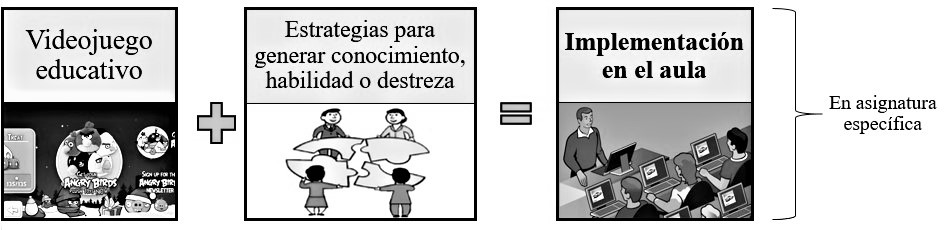
\includegraphics[width=0.85\textwidth]{Fig5.jpg}
 \caption{Diseño de las intervenciones en el aula basada en videojuegos educativos.}
 \label{fig05}
 \source{Elaboración propia.}
\end{figure}

\subsection{Discusión del objetivo 4. Limitaciones y proyecciones declaradas en los estudios}\label{sec-conclusao}

\subsubsection{Discusión respecto a los resultados de las limitaciones declaradas en los estudios}
Los resultados respecto a la limitación declarada en los estudios, identificó que 5 de ellos no las reportaron. De los 14 restantes que si las manifestaron, se reconocieron un total de 21 limitaciones, pues algunos expusieron más de una, lo que permitió detectar que los trabajos, presentan dificultades con la propia intervención realizada (42 \%), es decir, en su aplicación, diseño u otro algún otro elemento. Lo anteriormente mencionado, genera una discordancia respecto a los resultados encontrados, pues los estudios investigados con videojuegos educativos, por un lado, exponen como efectivas las intervenciones, pero por otro, las consideran una limitación. Atendiendo a esta declaración realizada por los propios autores, se debería mantener una cautelosa interpretación de los resultados, pues puede existir algún margen de error. Sin embargo, los autores \textcite{soto_estudios_2020}, no lo consideran como algo negativo, pues exponen que no existe un diseño perfecto en materia investigativa, y que el indicar las limitaciones metodológicas corresponde a una buena práctica, pues es la única forma de entregar conocimiento a quienes quieran replicar el estudio en un futuro.


\subsubsection{Discusión respecto de los resultados de futuras líneas de investigación declaradas en los estudios}
De acuerdo a las futuras líneas investigativas declaradas, en los resultados se identificó que 4 estudios no las publicaron. De los 15 restantes que si lo hicieron, se evidenció un total de 28 proyecciones. A raíz de esto, se detectó que las futuras líneas de investigación más declaradas se asocian a la misma intervención (38 \%) y al método del estudio (31 \%). Por lo anterior y tal como se ha señalado en estudios previos, es importante seguir avanzando en la mejora de las propuestas de intervención con videojuegos en contextos educativos, pues se deben ir ajustando a las necesidades que presenten las comunidades estudiantiles, pues es posible afirmar que sin duda los videojuegos constituyen en la actualidad una expresión clara de la cultura digital \cite{esnaola_mediacion_2018}. Por otra parte, futuros estudios podrían mejorar aspectos metodológicos gracias a las experiencias declaradas en las presentes investigaciones analizadas. De esta forma, se contribuye a la disminución de sesgos y dificultades que entorpezcan la generalización de los resultados. A raíz de esto, \textcite{islas_torres_implicacion_2017}, afirma que es necesario ahondar en investigaciones que den cuenta empírica de los alcances, limitaciones y prospectiva de las tecnologías en la educación, pues de esta forma se pueden ofrecer soluciones innovadoras que entreguen alternativas de calidad para el sistema educativo.

\section{Conclusiones}
De acuerdo a los resultados obtenidos y la discusión realizada, se pueden extraer las siguientes conclusiones principales que responden a los objetivos de la investigación:

\begin{enumerate}
    \item En relación a la descripción de los participantes, se encontró que en los países europeos y específicamente en España, es donde más se desarrollan intervenciones con videojuegos educativos en el nivel de secundaria, hallazgo que se contrapone a la escasa implementación dentro de Latinoamérica. Es por esto, que futuras investigaciones podrían apuntar incluir este tipo de tecnologías contextualizadas a la realidad del territorio latinoamericano. Además, se tiende considerar muestras pequeñas, para ser estudios mayoritariamente cuantitativos o mixtos, lo que genera una problemática, pues evidencia poca representatividad. Esto, es un elemento importante a considerar, pues los resultados pueden variar de acuerdo al tamaño muestral.
    \item En cuanto a las características de la variable independiente, se puede afirmar que, dentro de las intervenciones con videojuegos educativos en el nivel de secundaria, predominan las estrategias pedagógicas relacionadas con la asignatura de matemáticas. Esto revela, la escasa promoción de la herramienta tecnología en el área humanista y refleja una necesidad de poder indagar en el uso de videojuegos que aporten al desarrollo de competencias de comprensión e interpretación en los diversos subsectores de aprendizaje. De esta forma, se podría apreciar los beneficios de manera global en el sistema escolar secundario.
    \item De acuerdo con la efectividad de los videojuegos se puede afirmar que estos son efectivos tanto para el desarrollo cognitivo como para las habilidades socioemocionales. La clave está en la vinculación con una adecuada estrategia pedagógica al ámbito específico al cual se quiera integrar. Es por esto, que las universidades deberían incluirlos dentro de la formación inicial docente, pues existiría una mayor promoción de este recurso tecnológico en el aula, generando como consecuencia, un mayor alcance en el alumnado de los requerimientos necesarios para el siglo XXI.
    \item Finalmente, respecto a las limitaciones y proyecciones declaradas, se afirma que ambas manifiestan problemáticas y mejoras en la misma intervención. A pesar de que ninguna investigación es perfecta, siempre debe existir una muy buena previa planificación del diseño, método, instrumento y variables a tratar dentro de la intervención con videojuegos educativos, para que, de este modo, se pueda aplicar al aula con resultados positivos para el proceso socio cognitivo de los estudiantes. Es por esto que los hallazgos del presente estudio, podría ayudar a futuros investigadores a organizar mejor sus estudios.
\end{enumerate}

\section{Limitaciones del estudio}
Las limitaciones del presente proyecto de tesis se relacionan con la identificación de investigaciones registradas en solo tres bases de datos y en dos idiomas (inglés/ español), lo que puede ser un obstáculo para encontrar un mayor número de investigaciones empíricas relacionadas con las intervenciones de videojuegos educativos en el nivel de secundaria. Además, solo se llevó a cabo un estudio descriptivo – interpretativo, porque los objetivos propuestos responden a estos elementos. Sin embargo, se podría haber incluido un meta–análisis, para que la investigación tuviera una mayor consistencia y precisión en los resultados.

\section{Proyecciones y futuras de líneas de investigación del estudio}
En relación con las proyecciones de esta tesis, se establece la necesidad de mejorar los algoritmos de búsqueda e incluir más bases de datos, para poder ampliar la muestra. También se podría realizar un análisis comparativo entre las intervenciones educativas de diferentes niveles, para ver cuáles son las diferencias y similitudes que se obtienen según el avance curricular del estudiante. Finalmente, se espera que, en base a los hallazgos del estudio, se pueda desarrollar una intervención educativa con videojuegos que contemple algún país latinoamericano, diferentes asignaturas de aplicación y una mayor cantidad de sesiones y participantes, pues se ha detectado un vacío de conocimiento en esos ámbitos.

\section{Agradecimientos}
La presente investigación se encuentra vinculada al Proyecto Fondecyt regular 1191891, titulado \textit{Integración de tecnologías inmersivas en educación. Mecanismos de aprendizaje y prácticas educativas desde la formación de profesores}.


\printbibliography\label{sec-bib}
% if the text is not in Portuguese, it might be necessary to use the code below instead to print the correct ABNT abbreviations [s.n.], [s.l.]
%\begin{portuguese}
%\printbibliography[title={Bibliography}]
%\end{portuguese}


%full list: conceptualization,datacuration,formalanalysis,funding,investigation,methodology,projadm,resources,software,supervision,validation,visualization,writing,review
\begin{contributors}[sec-contributors]
\authorcontribution{Paula Rojas-García}[conceptualization,datacuration,writing]
\authorcontribution{Fabiola Sáez-Delgado}[conceptualization,datacuration,methodology,visualization,supervision,writing]
\authorcontribution{María Graciela Badilla-Quintana}[conceptualization,supervision]
\authorcontribution{Laura Jiménez-Pérez}[review]
\end{contributors}

%Os autores ainda não enviaram os dados.


\end{document}

